\section{Experimental Setup}
\label{sec:experimental_setup}

\looseness=-1
We evaluate how prompt schema size and inter-type confusability affect zero-shot LLM extraction across three information extraction tasks and four datasets: named entity recognition (NER), sentence-level relation extraction (RE), document-level RE, and event detection (ED).

\begin{figure*}[t]
\centering
\begin{minipage}[t]{0.48\textwidth}
\centering
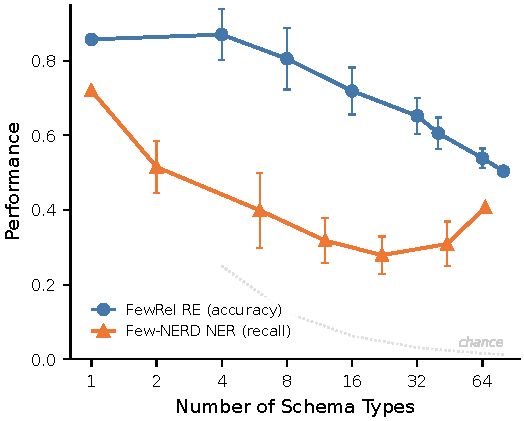
\includegraphics[width=\linewidth]{../../figures/paper/fig_count_curves.pdf}
\end{minipage}
\hfill
\begin{minipage}[t]{0.48\textwidth}
\centering
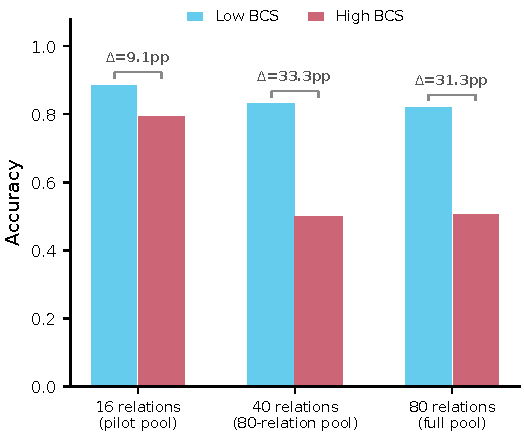
\includegraphics[width=\linewidth]{../../figures/paper/fig_bcs_scaling.pdf}
\end{minipage}
\caption{\textbf{(a)} Count-degradation curves. Error bars: $\pm 1$ standard deviation (SD) across 3 batch-composition seeds $\times$ 25 batches. RE declines monotonically; NER shows a U-shape. Rightmost points are full-schema (negligible sampling variance). \textbf{(b)} Illustrative BCS-controlled FewRel accuracy: each bar represents one extreme-BCS batch per condition. Slopes are consistent across pool conditions ($p = 0.60$); wider BCS range at 80 relations produces larger gaps. Statistical evidence is provided by the pooled regression (\S\ref{sec:bcs_controlled}, semipartial $R^2 = 0.273$, $n = 204$).}
\label{fig:main_results}
\end{figure*}

\subsection{Tasks and Datasets}
\label{sec:datasets}

\paragraph{Few-NERD (NER).}
\looseness=-1
Few-NERD \citep{fewnerd-2021} provides 66 fine-grained entity types organized into 8 coarse categories (person, location, organization, building, art, product, event, other). The dataset spans diverse domains. We sample 1{,}000 instances uniformly from the test set; type frequency follows the natural long-tail distribution of Few-NERD. Evaluation uses token-level text matching. Pairwise analysis covers 1{,}953 type pairs with non-zero co-occurrence out of $\binom{66}{2}=2{,}145$ possible pairs.

\paragraph{FewRel (RE).}
\looseness=-1
FewRel \citep{fewrel-2018} contains 80 relation types sourced from Wikidata. Since the validation split covers only 16 relations, we combine the training and validation splits to obtain the full 80-relation pool required for schema-scale experiments. We sample 1{,}000 balanced instances (12--13 per relation type, stratified to ensure equal representation). A held-out validation confirms SCS--confusion generalization across the split boundary (Appendix~\ref{app:scs-heldout-validation}). Each instance provides a sentence with marked head and tail entities; the task is to classify the relation. FewRel's balanced design (700 instances per relation type) eliminates type frequency as a potential confound; this balance makes it the primary dataset for BCS analysis. Contamination analysis (Appendix~\ref{app:split-origin}) shows extraction difficulty correlates inversely with training-set prevalence, and BCS effects are unchanged when controlling for contamination.

\paragraph{DocRED (Document-level RE).}
\looseness=-1
DocRED \citep{docred-2019} contains 96 relation types sourced from Wikidata, evaluated at the document level where entity pairs may span multiple sentences. We sample 1{,}000 instances balanced across 96 relation types ($\sim$10 per type) from the DocRED development set. The task is formulated identically to FewRel: given a document with marked head and tail entities, classify the relation. We use the development set, as DocRED test labels require submission to a hidden evaluation server. DocRED extends the RE evaluation to a larger schema (96 vs.\ 80 types) and document-level context, testing whether confusability effects persist under longer input contexts and cross-sentence reasoning.

\paragraph{MAVEN (ED).}
MAVEN \citep{maven-2020} defines 168 event types derived from the FrameNet ontology; all types belong to a single ontology (FrameNet), so this is a same-domain schema. We use the validation set (8{,}042 sentences containing 18{,}904 event mentions) for evaluation, as test set labels are not publicly available. The task requires both trigger identification and event type classification. MAVEN serves a supplementary role: its same-domain schema produces centrality confounds at the batch level (\S\ref{sec:centrality_confound}), and its compressed BCS range (0.87--0.97) limits the variance available for regression analysis.

Table~\ref{tab:datasets} summarizes the dataset statistics, including the Schema Confusability Score (SCS) ranges defined in \S\ref{sec:scs}.

% Table 1 (tab:datasets) moved to end of related_work.tex for page-3 placement

\subsection{Schema Confusability Score (SCS)}
\label{sec:scs}

\looseness=-1
We define the Schema Confusability Score (SCS) to quantify semantic overlap between types in a schema. Given a type $t$ with name string $\text{name}(t)$, an embedding function $\text{embed}(\cdot)$ maps the type name to a vector representation. The \textbf{pairwise SCS} between types $t_i$ and $t_j$ is:
{\small
\[
\text{SCS}(t_i, t_j) = \cos\bigl(\text{embed}(\text{name}(t_i)),\; \text{embed}(\text{name}(t_j))\bigr)
\]
}

We use mean pairwise SCS as the default BCS aggregation; max-based BCS yields directionally consistent results (Appendix~\ref{sec:appendix_bcs_sensitivity}, Table~\ref{tab:bcs_aggregation}). BCS captures confusability-specific signal beyond type composition (Appendix~\ref{app:bcs-composition}).

For a batch of types $B = \{t_1, \ldots, t_k\}$, the \textbf{Batch Confusability Score (BCS)} aggregates all pairwise similarities:
\[
\text{BCS}(B) = \frac{1}{\binom{k}{2}} \sum_{i < j,\; t_i, t_j \in B} \text{SCS}(t_i, t_j)
\]

\looseness=-1
We compute SCS with two embeddings: (1)~Qwen3-32B \citep{qwen3-2025} hidden-state representations (5{,}120-d) and (2)~all-MiniLM-L6-v2 \citep{minilm-2020,sentence-bert-2019}, a 384-d sentence encoder. MiniLM is the primary BCS embedding; cross-embedding consistency holds on all datasets, with MiniLM yielding equal or stronger correlations (Appendix~\ref{sec:appendix_bcs_sensitivity}). Few-NERD uses Qwen3 because its fine-grained same-category pairs require the higher-dimensional space. Name-only SCS yields equivalent predictive accuracy to name+definition (Appendix~\ref{app:scs-ablation}).

\paragraph{SCS as a lightweight proxy.}
\label{sec:scs-validation}
SCS is a pre-hoc proxy computable without running extraction; pairwise correlations with observed type confusion are reported in \S\ref{sec:pairwise}. SCS does not capture context-dependent disambiguation or mention-level ambiguity; these contribute to residual variance.

\begin{figure}[t]
\centering
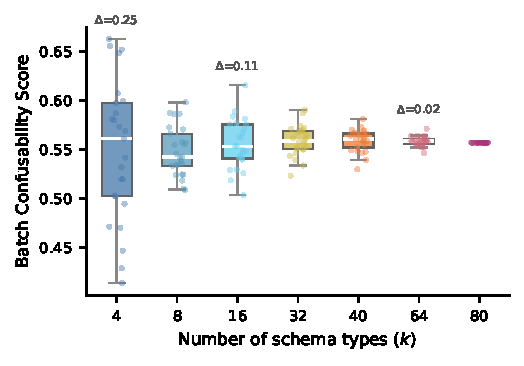
\includegraphics[width=\columnwidth]{../../figures/paper/fig_bcs_scatter.pdf}
\caption{BCS range compression on FewRel: as type count $k$ increases, achievable BCS range narrows ($\Delta{=}0.25$ at $k{=}4$ to $\Delta{<}0.01$ at $k{=}80$), limiting power to detect confusability effects without extreme-BCS construction (\S\ref{sec:exp_design}). Each point is one of 25 random batches; boxes show IQR.}
\label{fig:bcs_range}
\end{figure}

\subsection{Experimental Design}
\label{sec:exp_design}

We conduct two complementary experiments.

\paragraph{Experiment 1: Count Curves.}
\looseness=-1
We vary the number of types presented in the prompt schema to measure performance as a function of schema size. For each count level, we sample 25 random type batches for Few-NERD and FewRel (5 for DocRED and MAVEN)\footnote{DocRED and MAVEN use fewer batches due to higher per-batch evaluation cost (document-level RE and 8{,}042 sentences, respectively).} and evaluate against the same 1{,}000-sample pool. For NER and ED, all samples are evaluated in every batch; for RE, each batch evaluates only the subset whose gold relation appears in the candidate set ($k/K$ of the pool, where $K$ is the total number of types), so effective sample size scales with count. At count${}=1$, every type is evaluated individually as a solo baseline. The remaining count levels follow natural partition points in each schema's type hierarchy rather than uniform spacing: \{2, 6, 12, 22, 44, 66\} for Few-NERD, \{4, 8, 16, 32, 40, 64, 80\} for FewRel, \{4, 8, 16, 32, 64, 96\} for DocRED, and \{6, 12, 22, 44, 64\} for MAVEN.

\paragraph{Experiment 2: BCS-Controlled.}
\looseness=-1
We fix type count and vary BCS to isolate confusability from schema size. For each count level, we construct one low-BCS batch, one high-BCS batch, and 25 random batches (27 total). We construct extreme batches via greedy search over the pairwise SCS matrix. The low-BCS batch starts from the least-similar type pair and iteratively adds the type with lowest maximum similarity to already-selected types; the high-BCS batch mirrors this with maximum similarity. This design is motivated by BCS range compression: random batches exhibit narrowing BCS variance at higher counts ($\Delta = 0.25$ at $k{=}4$ vs.\ $< 0.01$ at $k{=}80$; Figure~\ref{fig:bcs_range}), limiting statistical power to detect confusability effects without extreme-BCS construction. We evaluate on Few-NERD (count$\,\in\{6, 12\}$), FewRel (count$\,\in\{8, 16\}$, both 16-relation (pilot) and 80-relation pools), and DocRED (count$\,\in\{16, 32\}$). Within-pool 16-relation subsets from the 80-relation pool isolate confusability from pool composition. MAVEN results are reported separately due to a centrality confound (\S\ref{sec:centrality_confound}).

\subsection{Evaluation Metrics}
\label{sec:metrics}

\textbf{NER}: text-match F1 (exact string + type match). \textbf{RE}: accuracy (exact relation label match; each batch evaluates only samples whose gold relation is among the candidates; \texttt{none} responses scored as incorrect). \textbf{ED}: relaxed F1 (token overlap + correct event type).


\subsection{Model and Inference}
\label{sec:model}

\looseness=-1
We use Qwen3-32B-FP8 \citep{qwen3-2025} served via vLLM v0.20.2 \citep{vllm-2023} on a single NVIDIA RTX PRO 6000 GPU (96\,GB) with greedy decoding (temperature${}\,=\,0$, seed 42). Two NER/ED prompt versions are evaluated: v1 requests character offsets; v2 adds format constraints that double precision with minimal recall loss. RE uses a single prompt version throughout (templates and type definitions in Appendix~\ref{sec:appendix_prompts}). The BCS--accuracy relationship is format-independent: constrained and unconstrained decoding yield identical correlations (Appendix~\ref{app:format-independence}). Cross-model validation uses Meta-Llama-3.1-70B-Instruct (FP8) and Meta-Llama-3.1-8B-Instruct \citep{llama3-2024}. Single-seed greedy decoding substantially reduces model-level randomness (residual SD${}\,=\,0.88$\,pp; Appendix~\ref{app:variance-decomposition}); bootstrap CIs capture batch-composition variance ($B{=}10{,}000$ pairwise; $B{=}1{,}000$ batch-level). Total computation is ${\sim}$72 GPU-hours on a single RTX PRO 6000.
